\documentclass[%
%oneside,                 % oneside: electronic viewing, twoside: printing
%$final,                   % draft: marks overfull hboxes, figures with paths
10pt]{article}

\listfiles               %  print all files needed to compile this document

\usepackage{relsize,makeidx,color,setspace,amsmath,amsfonts,amssymb}
\usepackage[table]{xcolor}
\usepackage{bm,ltablex,microtype}
\usepackage{graphicx}

\usepackage[T1]{fontenc}
%\usepackage[latin1]{inputenc}
\usepackage{ucs}
\usepackage[utf8x]{inputenc}

\usepackage{lmodern}

% Hyperlinks in PDF:
\definecolor{linkcolor}{rgb}{0,0,0.4}
\usepackage{hyperref}
\hypersetup{
    breaklinks=true,
    colorlinks=true,
    linkcolor=linkcolor,
    urlcolor=linkcolor,
    citecolor=black,
    filecolor=black,
    %filecolor=blue,
    pdfmenubar=true,
    pdftoolbar=true,
    bookmarksdepth=3   % Uncomment (and tweak) for PDF bookmarks with more levels than the TOC
    }
%\hyperbaseurl{}   % hyperlinks are relative to this root

% Tricks for having figures close to where they are defined:
% 1. define less restrictive rules for where to put figures
\setcounter{topnumber}{2}
\setcounter{bottomnumber}{2}
\setcounter{totalnumber}{4}
\renewcommand{\topfraction}{0.95}
\renewcommand{\bottomfraction}{0.95}
\renewcommand{\textfraction}{0}
\renewcommand{\floatpagefraction}{0.75}
% floatpagefraction must always be less than topfraction!
% 2. ensure all figures are flushed before next section
\usepackage[section]{placeins}
% 3. enable begin{figure}[H] (often leads to ugly pagebreaks)
%\usepackage{float}\restylefloat{figure}

\usepackage[framemethod=TikZ]{mdframed}


\setcounter{secnumdepth}{3}
\setcounter{tocdepth}{3}
\begin{document}

\thispagestyle{empty}

\begin{center}
{\LARGE\bf
\begin{spacing}{1.25}
Machine Learning and Artificial Intelligence activities at FRIB
\end{spacing}
}
\end{center}

\tableofcontents
\newpage

\section{Explanation}


The purpose of this document is to collect information about the  competence  in the area of ML/AI at FRIB Laboratory. This is important, e.g., for the upcoming \href{https://www.jlab.org/conference/AI2020}{\it AI FOR NUCLEAR PHYSICS WORKSHOP} at JLab, March 4-6, 2020 and other related  activities.


\subsection{Description of individual entries}
Please format your entry (1 entry per page) according to the following template:

\vspace{5mm}
\noindent
\fbox{\begin{minipage}{0.98\linewidth}
{\bf Topic} (in subsubsection title)
\begin{description}
\item[Participants] List local faculty/staff, research associates (p), students (g,u). External collaborators should be listed as co-authors in references.
\item[Description] Provide a short paragraph ($<$600 characters; think of a PRL abstract) describing the ML/AI aspects of the project.
\item[FRIB relevance] ($<$600 characters) 
\item[Outcomes] List instrumentation outcomes, if any. Provide your published/submitted/anticipated papers with hyperlinks 
\end{description}
You are encouraged to provide a figure below the description.
\end{minipage}}

\section{Machine Learning and AI in Nuclear Physics}


Artificial intelligence (AI)-based techniques, particularly in machine
learning (ML) and optimization, are increasingly being used in many areas
of experimental and theoretical physics to facilitate discovery,
accelerate data analysis and modeling efforts, and bridge different
physical and temporal scales in numerical models.
The large amount of degrees of freedom pertain to both theory and experiment in nuclear physics. With increasingly complicated experiments that produce large amounts data, automated classification of events becomes increasingly important. 
Artificial intelligence and Machine Learning   techniques are proving to be powerful tools for advancing our
understanding of the physics from complicated nuclear systems. 



\subsection{Types of Machine Learning}



The approaches to machine learning are many, but are often split into two main categories. 
In \emph{supervised learning} we have a situation with known input and output data that we want to reproduce with a given model, letting the given machine learning algorithm deduce the eventual logic behind our data. On the other hand, \emph{unsupervised learning}
is a method for finding patterns and relationship in data sets without any prior knowledge of the system.
Some authors also operate with a third category, namely \emph{reinforcement learning}. This is a paradigm 
of learning inspired by behavioural psychology, where learning is achieved by trial-and-error, 
solely from rewards and punishment.

Another way to categorize machine learning tasks is to consider the desired output of a system.
Some of the most common tasks are:

\begin{itemize}
  \item Classification: Outputs are divided into two or more classes. The goal is to   produce a model that assigns inputs into one of these classes. An example is to identify  digits based on pictures of hand-written ones. Classification is typically supervised learning.

  \item Regression: Finding a functional relationship between an input data set and a reference data set.   The goal is to construct a function that maps input data to continuous output values.

  \item Clustering: Data are divided into groups with certain common traits, without knowing the different groups beforehand.  It is thus a form of unsupervised learning.
\end{itemize}
These categories are all part of the broad spectrum of AI and ML techniques being studied at FRIB. 


\subsection{Acronyms of machine learning/statistical terms used}

We list here various acronyms used in the description of the different AI/ML projects.

\begin{description}
\item[AE] Auto encoders
\item[AI] Artificial intelligence
\item[BC] Bayesian calibration
\item[BM] Boltzmann machines/Reduced Boltzmann machines
\item[BMA] Bayesian model averaging
\item[BML] Bayesian machine learning
\item[BNN] Bayesian neural networks
\item[BS] Bayesian statistics
\item[CI] Credibility interval
\item[CL] Clustering
\item[CNN] Convolutional neural networks
\item[CoD] Coefficient of determination
\item[DL] Deep learning
\item[DRB] Decision trees, random forests and boosting
\item[ECP] Empirical coverage probability
\item[FS] Frequentist statistics
\item[GM] Graphical models
\item[GP] Bayesian Gaussian processes
\item[KR] Kernel regression
\item[LR] Logistic regression
\item[LSTM] Long short-term memory
\item[MCMC] Markov chain Monte Carlo
\item[ML] Machine learning
\item[NN] Neural networks
\item[PCA] Principal component analysis and dimensionality reduction techniques
\item[REG] Linear regression 
\item[RL] Reinforcement learning
\item[RNN] Recurrent neural networks
\item[SL] Supervised learning
\item[SVM] Support vector machines
\item[UQ] Uncertainty quantification
\item[VAE] Variational auto encoders
\end{description}

\clearpage
\newpage

\section{AI/ML projects at FRIB}

\subsection{Accelerators}

%%%%%%%%%%%%%%%%%%%%%%  Entry Begins %%%%%%%%%%%%%%%%%%%%%%%%%
\subsubsection{Add title}
\vspace{5mm}
\noindent
\fbox{\begin{minipage}{0.96\linewidth}
\begin{description}
%%%
\item[Participants:] 
%%%
\item[Description:]
%%%
\item[FRIB relevance:] 
%%%
\item[References:] {\it To be added}, in press/preparation/ or published 
\end{description}
%%%
\end{minipage}
}
\begin{figure}[htb!]
\centering
\caption{To be added}
\end{figure}
\clearpage
\newpage
%%%%%%%%%%%%%%%%%%%%%%  Entry Ends %%%%%%%%%%%%%%%%%%%%%%%%%

\subsection{Detectors}
\subsubsection{Gamma-ray Tracking}
\vspace{5mm}
\noindent
\fbox{\begin{minipage}{0.96\linewidth}
\begin{description}
%%%
\item[Participants:] D. Weisshaar, A. Gade, J. Chung
\item[Description:    ]
%%%
\item[FRIB relevance: Improvement  ] 
%%%
\item[References:] {\it To be added}, in press/preparation/ or published 
\end{description}
%%%
\end{minipage}
}
\begin{figure}[htb!]
\centering
\caption{To be added}
\end{figure}
\clearpage
\newpage


\subsection{Data Analysis and Statistical Analysis}

\subsubsection{Machine learning methods for track classification in the AT-TPC}

\vspace{5mm}
\noindent
\fbox{\begin{minipage}{0.96\linewidth}
\begin{description}
%%%
\item[Participants:] D. Bazin, M. Hjorth-Jensen
%%%
\item[Description:] We have implemented several  ML methods for event classification in the Active-Target Time Projection Chamber (AT-TPC) detector at NSCL. In particular we have implemented advanced convolutional AE NN to the analysis of two-dimensional projections of particle tracks
from a resonant proton scattering experiment on $^{46}$Ar.


%%%
\item[FRIB relevance:] We expect that many of the new FRIB experiments will produce large amounts of data. A class of detectors such as the AT-TPC is able to detect several reaction channels simultaneously. Extracting low cross section channels requires to classify the events of interest, which requires a large degree of automation. We expect that these techniques will play a central role at FRIB. 
%%%
\item[References:] {\it Machine learning methods for track classification in the AT-TPC},  M.P.Kuchera, R.Ramanujan, J.Z.Taylor, R.R.Strauss, D.Bazin, J.Bradt, R.M. Chen,
\href{https://doi.org/10.1016/j.nima.2019.05.097}{Nucl. Inst. Meth. A 940, 56 (2019)}
\end{description}
%%%
\end{minipage}
}
\begin{figure}[htb!]
\centering
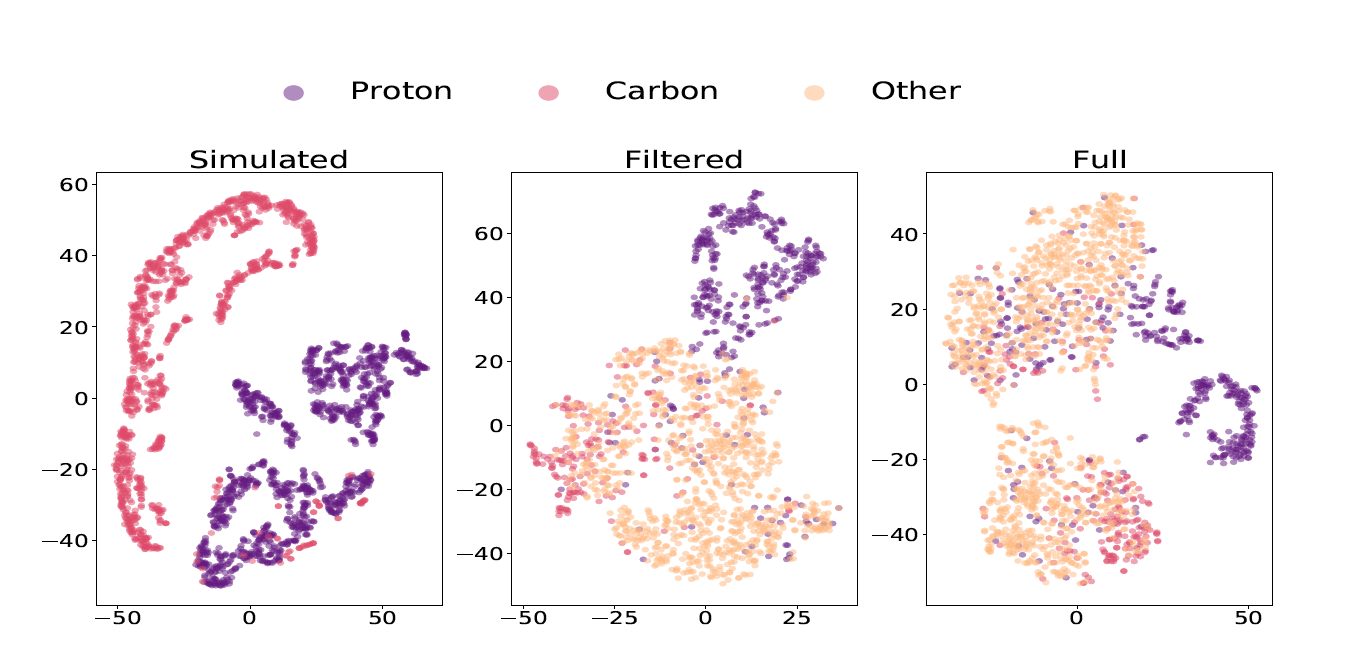
\includegraphics[width=\linewidth]{figures/attpc.png}
\caption{Visualization of the latent space from the VGG16 model on
three different data-sets.  The
axes have arbitrary non-informative units.}
\end{figure}
\clearpage
\newpage



\subsection{Basic Research}

\subsubsection{Bayesian Approach to Extrapolations of Nuclear Observables}
\vspace{5mm}
\noindent
\fbox{\begin{minipage}{\linewidth}
\begin{description}
%%%
\item[Participants:] L. Neufcourt (p), Y. Cao (s), W. Nazarewicz, and F. Viens (STT)
%%%
\item[Description:]  To improve the quality of model-based predictions of nuclear properties of rare isotopes far from stability, we consider the information contained in the residuals in the regions where the experimental information exist.  The emulators of  residuals and CIs defining theoretical error bars are constructed using  GP  and BNN.
%%%
\item[FRIB relevance:] The proposed Bayesian SL approach to extrapolation of nuclear model predictions can be useful for assessing the impact of current and future FRIB experiments. The new capability to evaluate residuals is also expected to impact research in the domains where experiments are currently impossible, for instance, in simulations of the astrophysical $r$ process.
%%%
\item[References:] {\it Bayesian approach to model-based extrapolation of nuclear observables}, L. Neufcourt, Y. Cao, W. Nazarewicz, and F. Viens, \href{https://journals.aps.org/prc/abstract/10.1103/PhysRevC.98.034318}{Phys. Rev. C 98, 034318 (2018)} (Editor's Suggestion).
\end{description}
%%%
\end{minipage}
}
\begin{figure}[htb!]
\centering
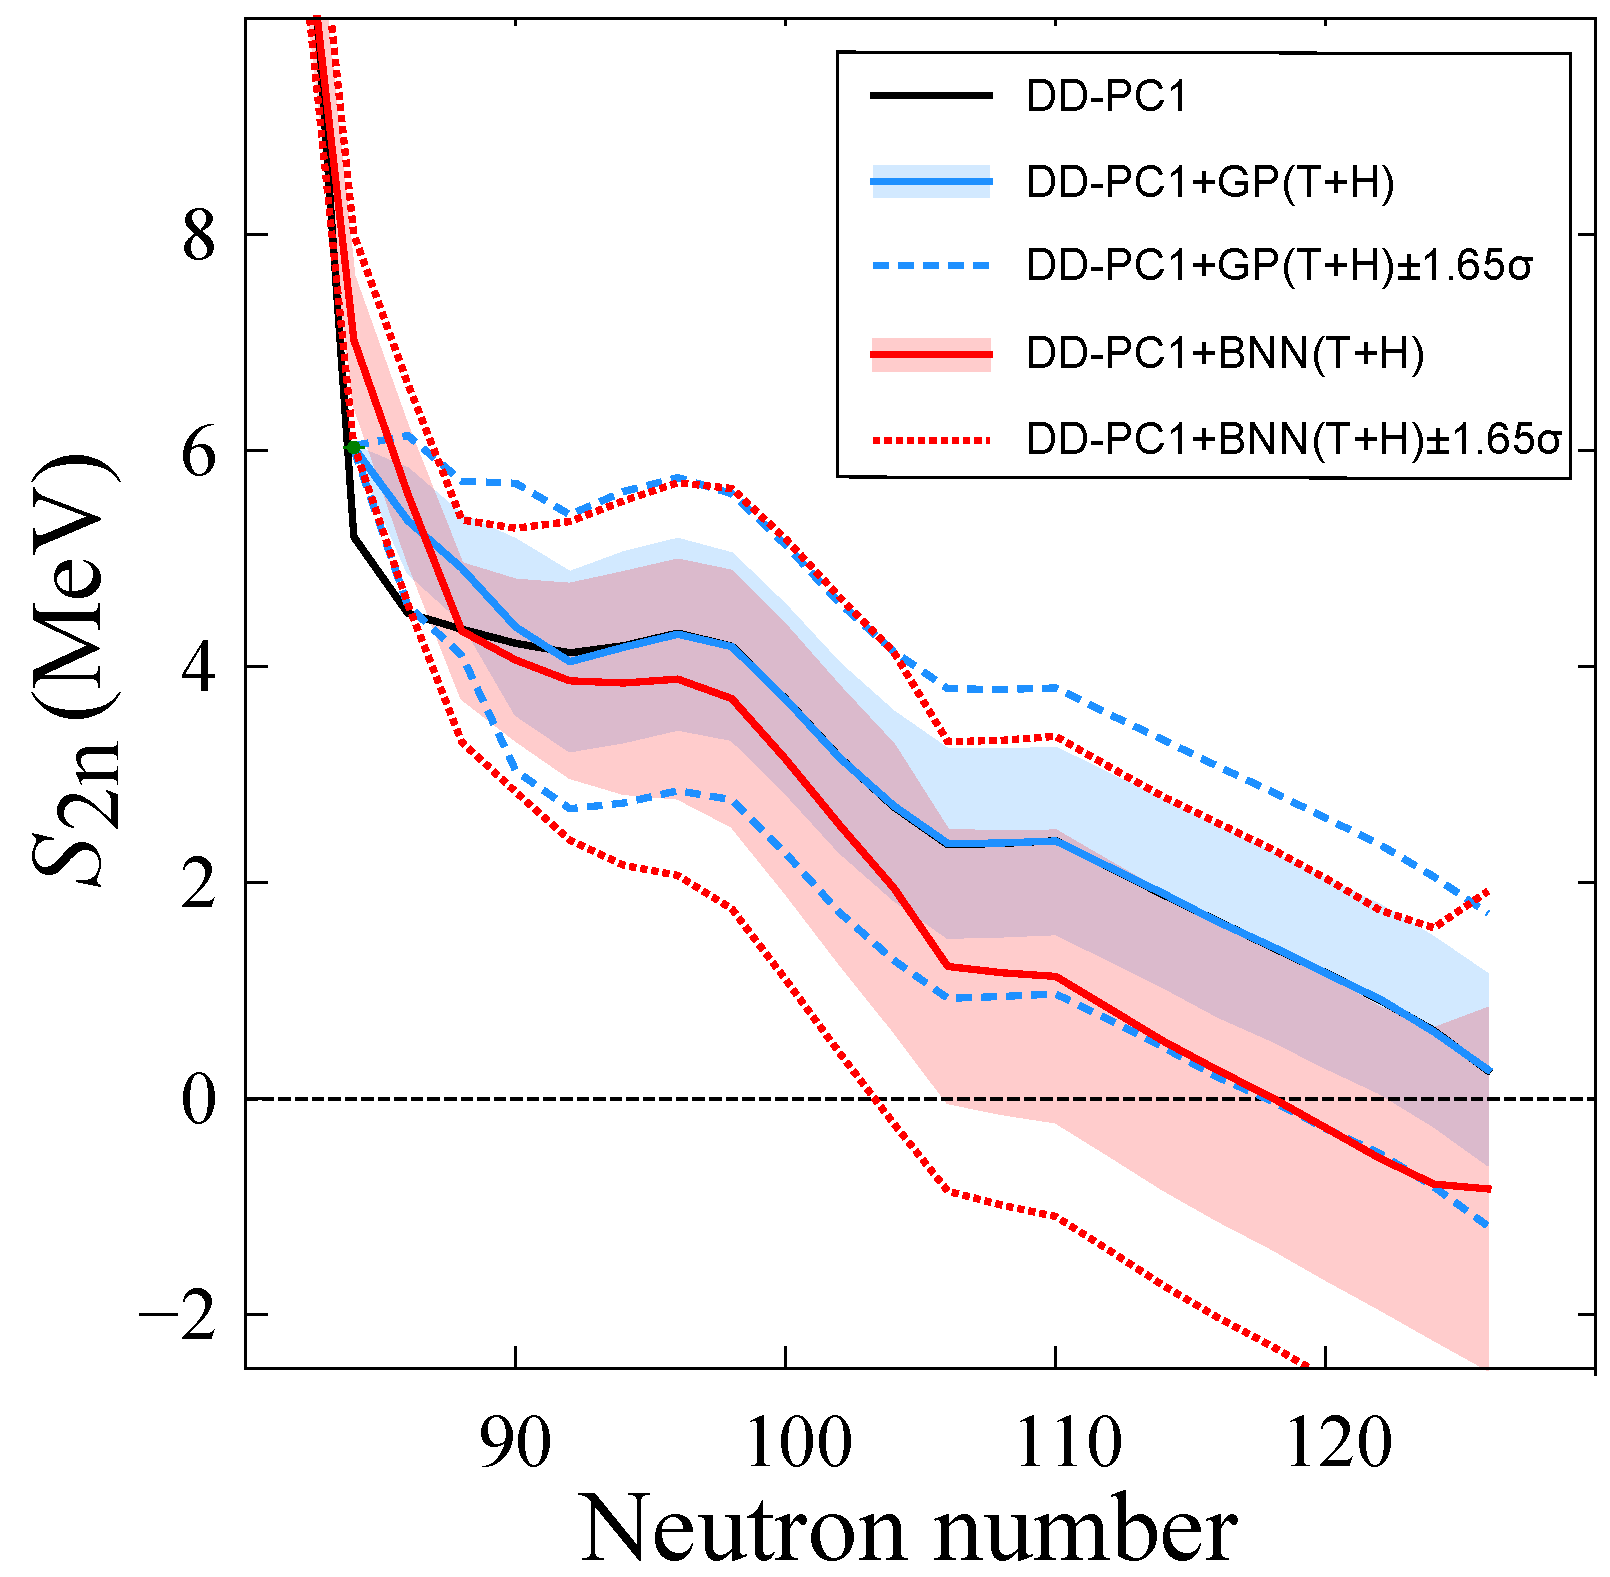
\includegraphics[width=0.63\linewidth]{figures/Sn-sep.pdf}
\caption{
Extrapolations of two-neutron separation energies for the even-even Sn chain
calculated  with DD-PC1 model  with statistical GP and BNN approaches.
One-sigma and 1.65-sigma CIs are marked.
}
\end{figure}

\clearpage
\newpage


\subsubsection{Nuclear Landscape with Bayesian Model Averaging}
\vspace{5mm}
\noindent
\fbox{\begin{minipage}{0.96\linewidth}
\begin{description}
%%%
\item[Participants:] L. Neufcourt (p), Y. Cao (g), S.A. Giuliani (p), W. Nazarewicz, and O.B. Tarasov
%%%
\item[Description:] We use microscopic nuclear global mass models and Bayesian SL methodology to provide quantified predictions of proton and neutron separation energies  as well as Bayesian probabilities of existence
 throughout the nuclear landscape all the way to the particle drip lines. To account for uncertainties, Bayesian GP are trained on the separation-energy residuals for each individual model, and the resulting  predictions are  combined via BMA. This framework allows to account for systematic and statistical uncertainties and propagate them to extrapolative predictions. 
%%%
\item[FRIB relevance:] Considering the anticipated  FRIB production rates and uncertainties of theoretical predictions, we identified  regions, reached by FRIB, that are crucial for constraining theoretical mass models.
%%%
\item[References:] {\it Beyond the proton drip line: Bayesian analysis of proton-emitting nuclei}, L. Neufcourt, Y. Cao, S. Giuliani, W. Nazarewicz,  E. Olsen, and O.B. Tarasov \href{https://journals.aps.org/prc/abstract/10.1103/PhysRevC.101.014319}{Phys. Rev. C 101, 014319 (2020)}; {\it Quantified limits of the nuclear landscape}, \href{https://arxiv.org/abs/2001.05924}{arXiv:2001.05924, submitted}.
\end{description}
%%%
\end{minipage}
}
\begin{figure}[htb!]
\centering
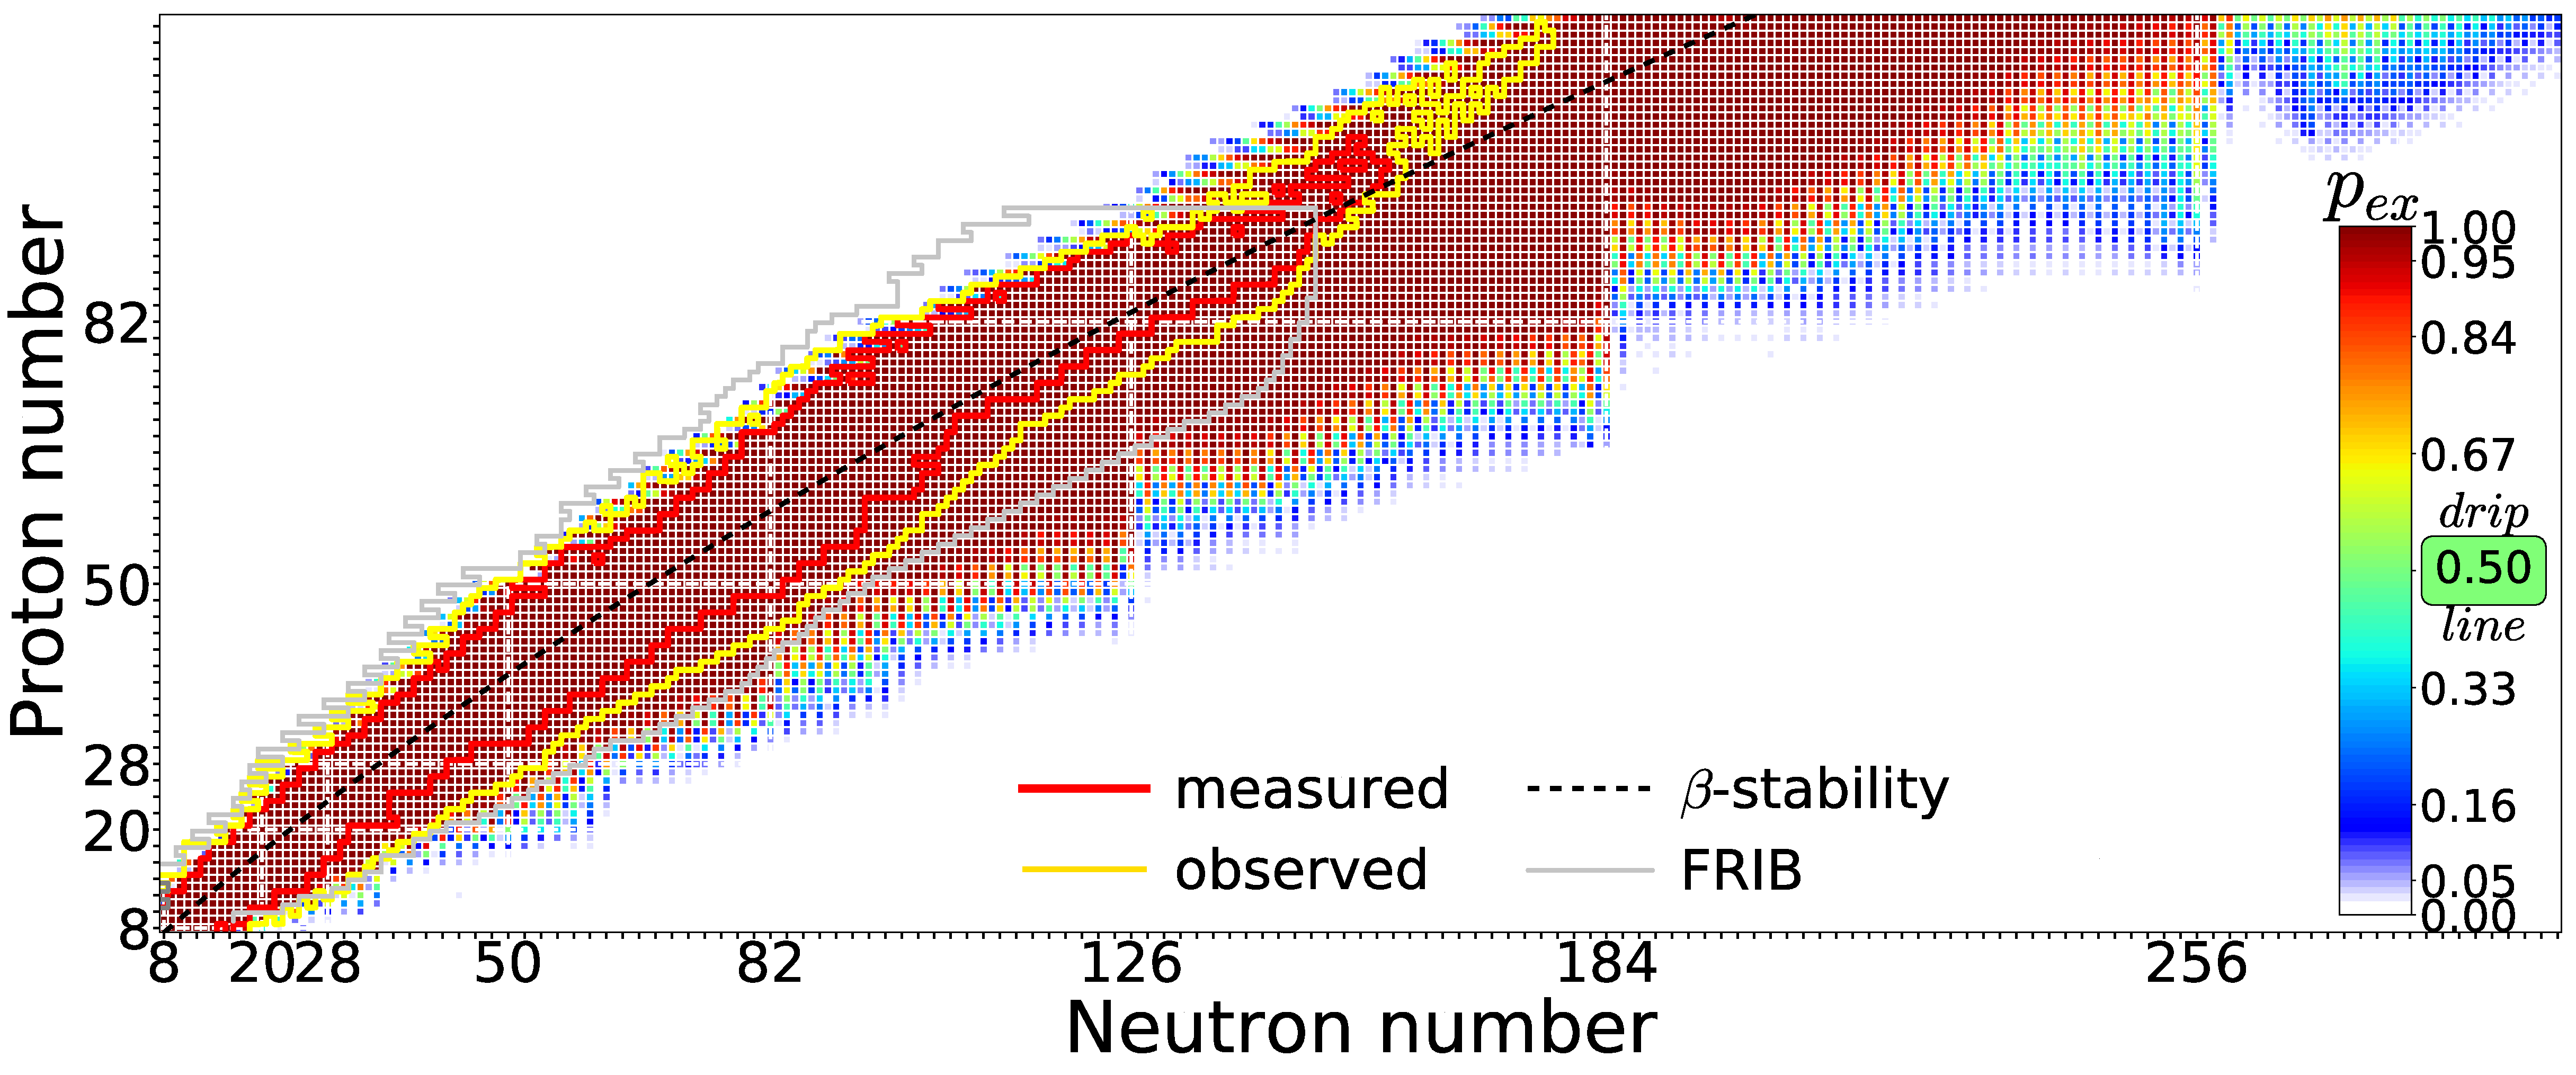
\includegraphics[width=\linewidth]{figures/Landscape.pdf}
\caption{
The quantified  landscape of nuclear existence obtained in our BMA calculations. For every nucleus with $Z,N \ge 8$ and $Z\le 119$
the probability that  the nucleus is bound with respect to proton and neutron decay, is marked.
The domains of nuclei which have been experimentally observed and whose separation energies have been  measured (and  used for training) are indicated together with 
the experimental reach of  FRIB.
}
\end{figure}

\clearpage
\newpage




\subsubsection{Deep Learning and the Nuclear Many-Body Problem}
\vspace{5mm}
\noindent
\fbox{\begin{minipage}{0.96\linewidth}
\begin{description}
%%%
\item[Participants:] J. Butler (g), Jane Kim (g), O Udiani (g), S. Bogner, H. Hergert, and M Hjorth-Jensen
%%%
\item[Description:] ML methods make it possible to tackle the curse of dimensionality and allow us to model quantum mechanical systems with less a priori knowledge. For complex many-body systems like nuclei (especially those at the limits of stability) or nuclear matter, this is a very interesting avenue to explore.  We have recently applied DL methods --- particular RNNs, LSTM and KRR --- to Similarity
Renormalization Group flows and the solution of Coupled Cluster theory, with a great deal of success. Our preliminary studies hold great promise for handling systems with large numbers of particles (including nuclear matter) or basis states (e.g. due to deformation or continuum coupling).
%%%
\item[FRIB relevance:]  Theoretical studies of nuclei at the limits of stability are a great challenge due to the large number of degrees of freedom. These systems are highly relevant for the scientific program of FRIB. Our early results also suggest connections between RG methods and Deep Learning that will contribute to a better understanding of Machine Learning methods.
%%%
\item[References:] {\it Recurrent Neural Networks and the Nuclear Many-body Problem}, in preparation
\end{description}
%%%
\end{minipage}
}
\begin{figure}[htb!]
\centering
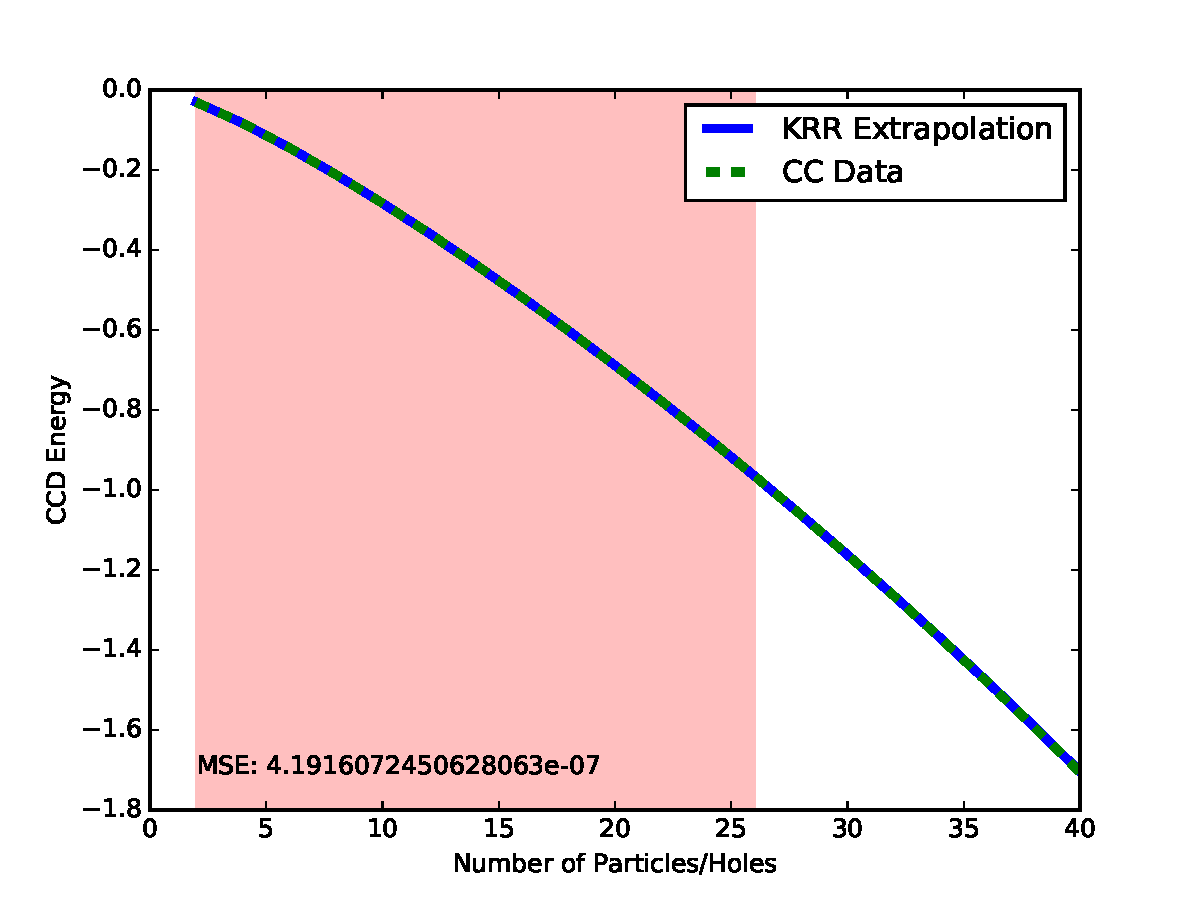
\includegraphics[width=0.75\linewidth]{figures/KRR_CC.pdf}
\vspace{-8pt}
\caption{Extrapolations to large numbers of interacting fermions for a pairing model using KRR methods on Coupled Cluster data.}
\end{figure}
\clearpage
\newpage

\subsubsection{Boltzmann Machines and the Nuclear Many-Body Problem}
\vspace{5mm}
\noindent
\fbox{\begin{minipage}{0.98\linewidth}
\begin{description}
%%%
\item[Participants:] J. Butler (g), Jane Kim (g), S. Bogner, and M Hjorth-Jensen
%%%
\item[Description:] We have recently started to explore several approaches based on DL algorithms, with an emphasis on NN and BM, with several promising results for interacting
many-fermion systems. Our applications
so far have been to systems of electrons confined to move in two or
three-dimensional regions (so-called quantum dots) and systems of
bosons (weakly and strongly interacting) using a mix of NN
based algorithms and variational quantum Monte Carlo approaches. We are in the process of extending these calculations
to nuclear physics problems.
%%%
\item[FRIB relevance:] The ability to study theoretically nuclei at the limits of stability is a great challenge due to the huge number of degrees of freedom. These systems are highly relevant for the scientific program of FRIB. 
%%%
\item[References:] {\it Solving Many-Body Problems with Boltzmann Machines}, in preparation
\end{description}
%%%
\end{minipage}
}
\begin{figure}[htb!]
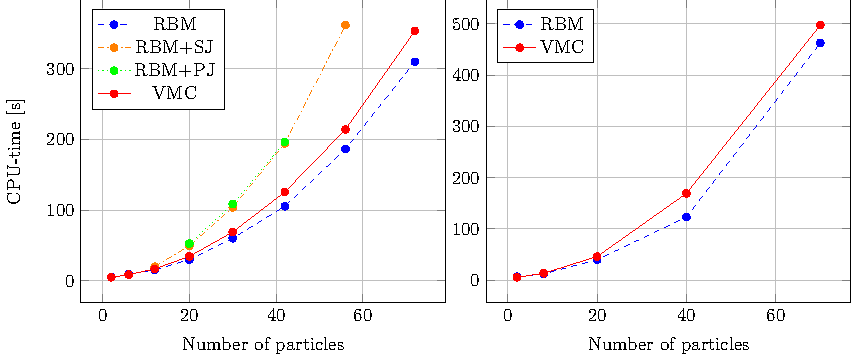
\includegraphics[width=\linewidth]{figures/quantumdots.pdf}
\caption{Ground state energies for systems of quantum dots.}
\end{figure}

\clearpage\newpage

\subsubsection{Emulators for the Nuclear Many-Body Problem}
\vspace{5mm}
\noindent
\fbox{\begin{minipage}{0.98\linewidth}
\begin{description}
%%%
\item[Participants:] D. Lee
%%%
\item[Description:] In applications of machine learning and uncertainty quantification to first principles nuclear many-body theory, one important tool is a fast and accurate emulator that removes the need for repeatedly performing computationally-expensive calculations.  We show that eigenvector continuation can fill this role quite nicely.  In addition to its applications as an emulator, eigenvector continuation can also be trained as a machine learning method for the quantum many-body problem using optimized variational subspaces. 
%%%
\item[FRIB relevance:] One of the fundamental challenges in FRIB science is understanding the connection between microscopic nuclear forces and nuclear structure.  Having a fast and accurate emulator makes it possible to apply machine learning and uncertainty quantification to uncover the correlations between nuclear forces and structure.
%%%
\item[References:] {\it Eigenvector Continuation as an Efficient and Accurate Emulator for Uncertainty Quantication in Nuclear Systems}, S. König, A. Ekström, K. Hebeler, D. Lee, and A. Schwenk, \href{https://arxiv.org/abs/1909.08446}{arXiv:1909.08446, submitted}.
\end{description}
%%%
\end{minipage}
}
\begin{figure}[htb!]
\centering
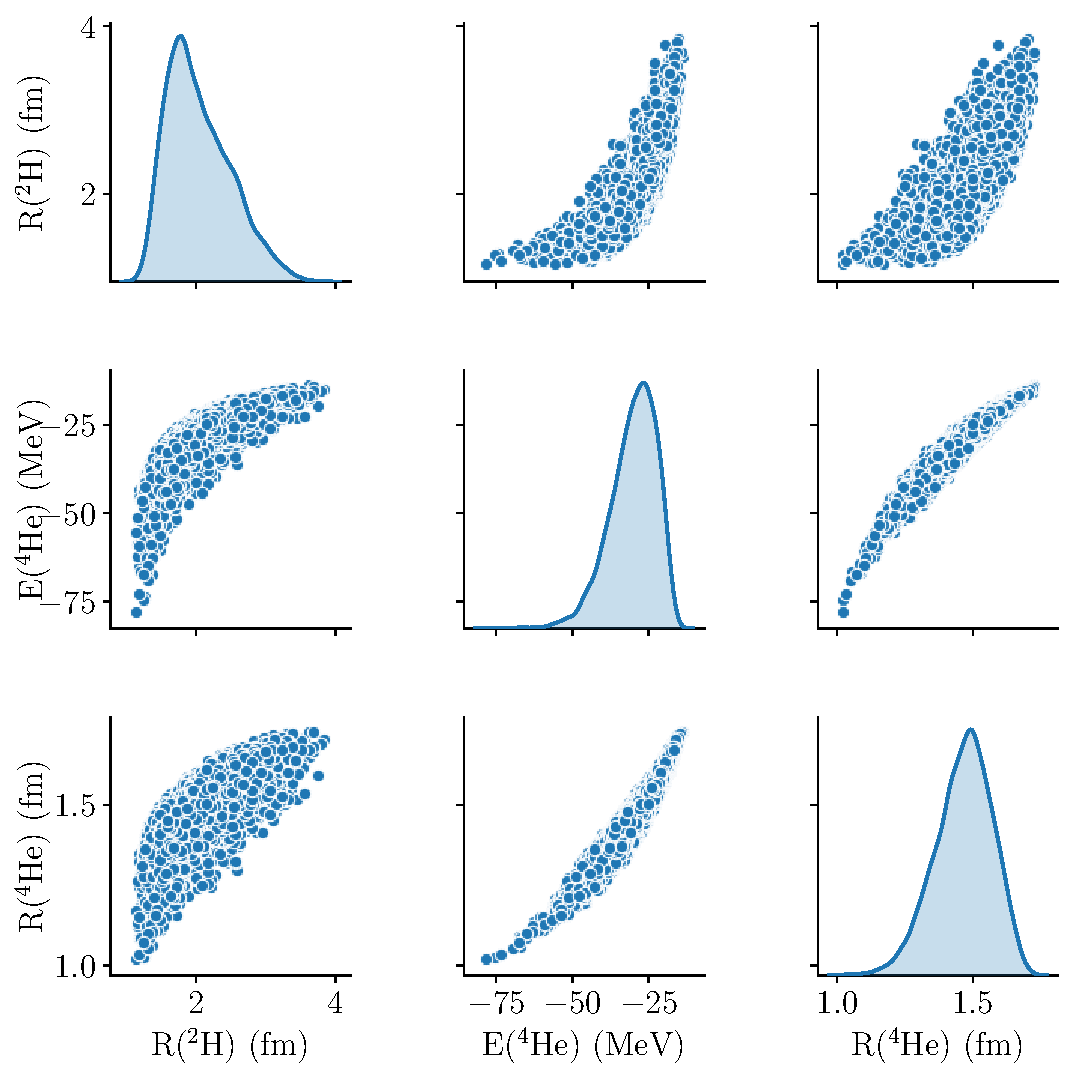
\includegraphics[width=8cm]{figures/few_body_grid_subset.pdf}
\caption{Correlations among several observables for $^2$H and $^4$He computed using eigenvector continuation.}
\end{figure}

\clearpage\newpage

\subsubsection{Machine Learning Multi-Nucleon Correlations}
\vspace{5mm}
\noindent
\fbox{\begin{minipage}{0.98\linewidth}
\begin{description}
%%%
\item[Participants:] J. Bonitati (g), G. Given (g), and D. Lee
%%%
\item[Description:] We are using BM to uncover and quantify multi-nucleon correlations in supercomputer lattice data obtained from lattice simulations of atomic nuclei.  The work involves the development of new algorithms to bypass the computational bottleneck of computing the overall normalization of the partition function and dealing with negative weight configuration produced in the quantum simulations.
%%%
\item[FRIB relevance:] We would like to understand the microscopic origins of nuclear clustering across the nuclear chart.  As the phenomenon of clustering is accentuated near open thresholds, these studies are of direct relevance to FRIB science.
%%%
\item[References:] {\it Machine Learning Multi-Nucleon Correlations from First Principles}, J. Bonitati, G. Given, Da. Lee, and D. Lee, in preparation.
\end{description}
%%%
\end{minipage}
}
\begin{figure}[htb!]
\centering
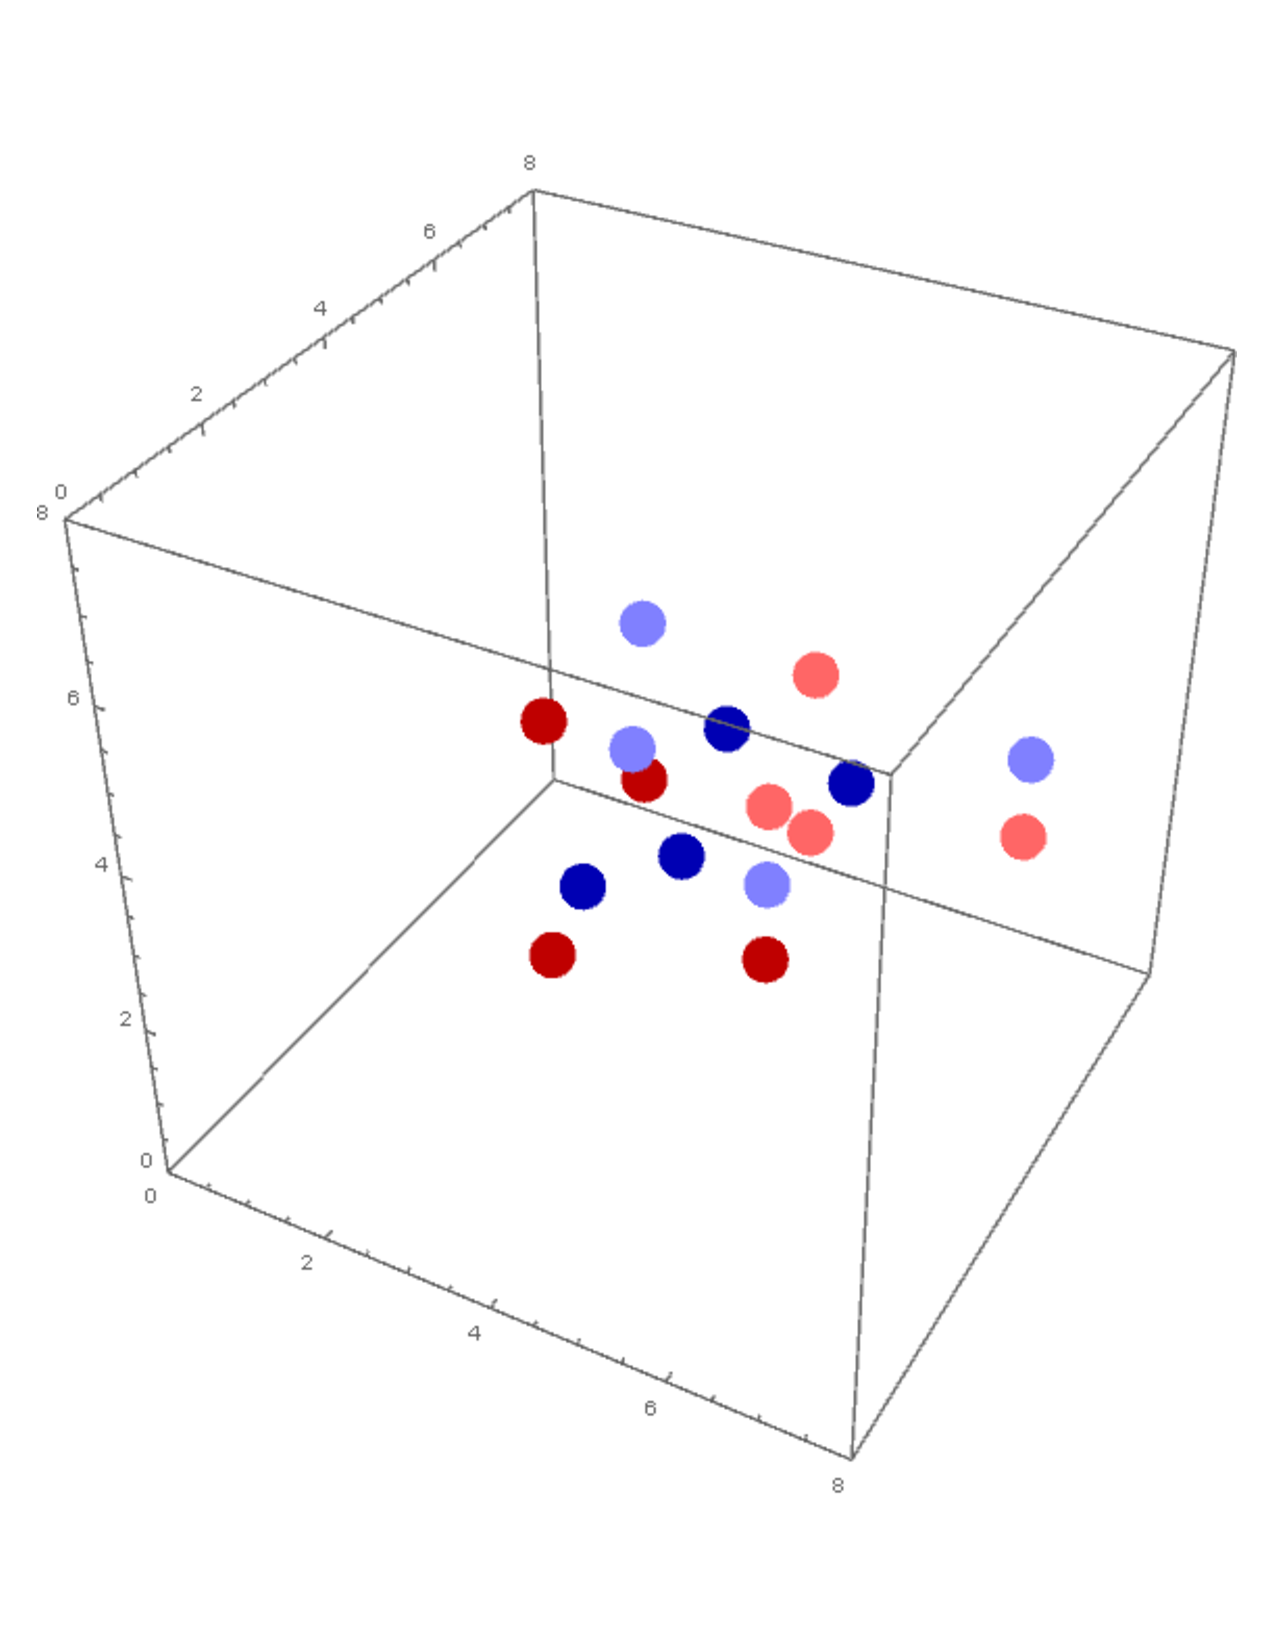
\includegraphics[width=7cm]{figures/training_data.pdf}
\caption{Sample training data used for machine learning multi-nucleon correlations in $^{16}$O.}
\end{figure}

\clearpage\newpage


\subsection{Applications}
\subsubsection{Add title}
\vspace{5mm}
\noindent
\fbox{\begin{minipage}{0.96\linewidth}
\begin{description}
%%%
\item[Participants:] Names%%%
\item[Description:]
%%%
\item[FRIB relevance:] 
%%%
\item[References:] {\it To be added}, in press/preparation/ or published 
\end{description}
%%%
\end{minipage}
}
\begin{figure}[htb!]
\centering
\caption{To be added}
\end{figure}
\clearpage
\newpage



\section{Education and Workforce}

AI, ML, statistical data analysis and related areas are expected to
play an ever-increasing role in many areas, from fundamental and
applied research at universities and national laboratories to
applications and developments in both the private and the public
sectors.
Developing basic research activities in these frontier
computational technologies is thus of strategic importance for our
society’s capability to address future scientific problems. Transfer
of knowledge to other disciplines and sectors, as well as developing
lasting collaborations with partners outside the traditional
university sector, are themes we expect will benefit society at large
and that will play central roles. Nuclear Physics keeps attracting many brilliant young researchers and providing our work force with these competences and skills for solving complicated physics problems is a compelling task for our community.


\begin{itemize}

\item In order to develop education and training efforts that target AI and ML related methods applied to Nuclear Physics, we  organized in 2019 a four day long  FRIB-TA workshop on ML methods in Nuclear physics at the NSCL/FRIB, with more than 100 participants.

\item In 2020 several of us (Bazin, Hjorth-Jensen and Liddick) will teach a three-week long Nuclear Talent course on Machine Learning and Data Analysis applied to nuclear physics. 

\item
We initiated the series of meetings on {\it Enhancing the interaction between nuclear experiment and theory through information and statistics} \href{https://iopscience.iop.org/journal/0954-3899/page/ISNET}{(ISNET)}.  The next ISNET-8 will be held at FRIB during  Dec. 14-17th, 2020.

\end{itemize}

\clearpage
\newpage

%%%%%%%%%%%%%%%%%%%%%%%%%%%%%% future %%%%%%%%%%%%%%%%%%%%%%%%%%%%%%%%%%%%%%%%%%%%
\section{Appendix: Anticipated projects}

Please format your entry (1 entry per page) according to the following template:

\vspace{5mm}
\noindent
\fbox{\begin{minipage}{0.98\linewidth}
{\bf Topic} (in subsubsection title)
\begin{description}
\item[Participants] List local faculty/staff, research associates (p), students (g,u). External collaborators should be listed as co-authors in references.
\item[Description] Provide a short paragraph ($<$600 characters; think of a PRL abstract) describing the ML/AI aspects of the project.
\item[FRIB relevance] ($<$600 characters) 
\item[Outcomes] List instrumentation outcomes, if any. Provide your published/submitted/anticipated papers with hyperlinks 
\end{description}
You are encouraged to provide a figure below the description.
\end{minipage}}



\end{document}
